\chapter{XÂY DỰNG HỆ THỐNG}
\label{chap:xaydung}

Chương này mô tả cách xây dựng hệ thống: thu thập và chia dữ liệu, gán nhãn, huấn luyện mô hình phát hiện, giao thức
so sánh hai họ kiến trúc, chọn thuật toán theo dõi và ghép các thành phần thành pipeline đếm xe. Toàn bộ mã nguồn viết
bằng Python, dùng các thư viện Ultralytics~\cite{ultralytics} (huấn luyện và theo dõi), Supervision~\cite{supervision}
(đếm qua vạch, vẽ kết quả), Transformers~\cite{transformers} (RT-DETRv2) và TrackEval~\cite{trackeval} (chấm theo dõi).

\section{Dữ liệu}

\subsection{Nguồn dữ liệu huấn luyện}

Không có bộ dữ liệu công khai nào khớp hoàn toàn với bài toán, nên đề tài gộp bảy nguồn, mỗi nguồn bù một điểm thiếu
của các nguồn còn lại (Bảng~\ref{tab:nguon-du-lieu}, Hình~\ref{fig:nguon-du-lieu}). Nhãn của mọi nguồn được đổi về
bốn lớp của đề tài theo tên lớp; riêng xe van trong VisDrone được gộp vào ô tô.

\begin{table}[H]
  \centering
  \caption{Các nguồn dữ liệu huấn luyện}
  \label{tab:nguon-du-lieu}
  \small
  \begin{tabularx}{\linewidth}{|p{3.3cm}|L|p{2.3cm}|p{2.1cm}|}
    \hline
    \thead{Nguồn} & \thead{Đặc điểm và cách dùng} & \thead{Dùng cho} & \thead{Giấy phép} \\ \hline
    vietnamese-vehicle v3~\cite{roboflow_vnvehicle} & Ảnh xe Việt Nam từ nhiều cảnh; nguồn duy nhất được chia ra cả
      val và test & Train, val, test & CC BY 4.0 \\ \hline
    vehicle-vietnam-cantho v19~\cite{roboflow_cantho} & Gần như một camera cố định ở Cần Thơ; lấy 300 ảnh & Train &
      CC BY 4.0 \\ \hline
    vehicle-detection v2~\cite{roboflow_indo} & Gần như một camera cố định; lấy 300 ảnh & Train & CC BY 4.0 \\ \hline
    VisDrone2019-DET~\cite{zhu2022visdrone} & Ảnh từ drone, rất nhiều xe máy nhỏ; chỉ lấy 909 ảnh có từ 10 xe máy trở
      lên & Train & Chỉ dùng cho nghiên cứu \\ \hline
    UVH-26~\cite{sharma2025uvh26} & Ảnh camera giao thông Bengaluru (Ấn Độ), khoảng 2.800 camera; lấy 2.000 ảnh,
      đổi 14 lớp về 4 lớp & Train & CC BY 4.0 \\ \hline
    Video ngã tư Hà Nội (YouTube, kênh Raw Street Capture 101) & 69 frame nhãn tự động (lặp 4 lần khi train) và 10
      frame val nhãn tay; 30 frame khác làm test & Train, val, test & Chỉ dùng học tập \\ \hline
    Video đường phố TP.HCM ban đêm (YouTube, kênh Midnight Soundscape) & 288 frame từ hai camera, nhãn tự động; chỉ
      có từ v6 & Train & Chỉ dùng học tập \\ \hline
  \end{tabularx}
\end{table}

\begin{figure}[H]
  \centering
  \begin{subfigure}{0.32\linewidth}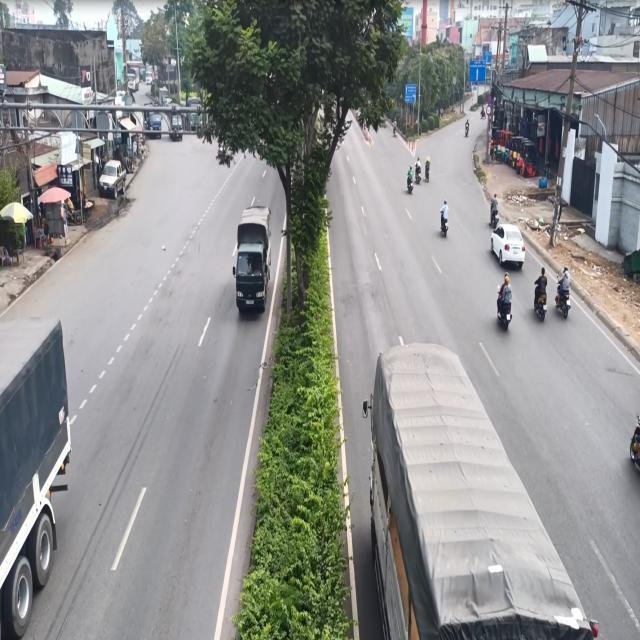
\includegraphics[width=\linewidth]{data_vnvehicle.jpg}\caption{vietnamese-vehicle}\end{subfigure}\hfill
  \begin{subfigure}{0.32\linewidth}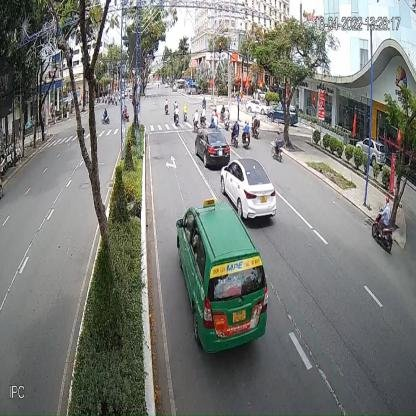
\includegraphics[width=\linewidth]{data_cantho.jpg}\caption{vehicle-vietnam-cantho}\end{subfigure}\hfill
  \begin{subfigure}{0.32\linewidth}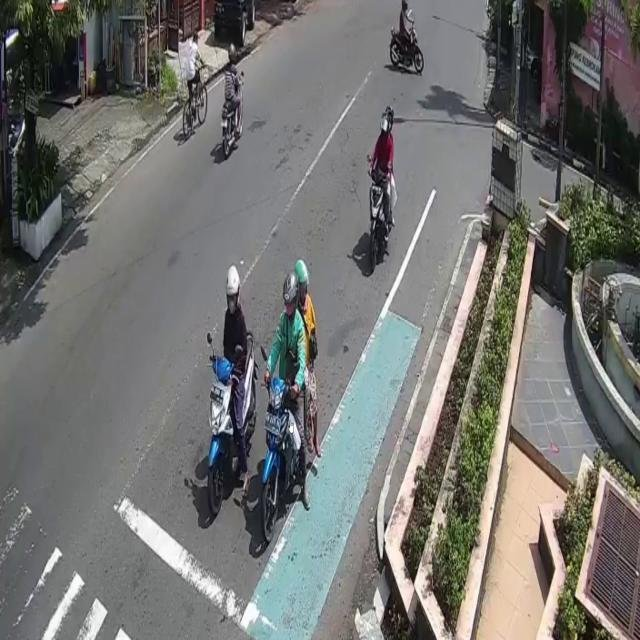
\includegraphics[width=\linewidth]{data_indo.jpg}\caption{vehicle-detection}\end{subfigure}\\[4pt]
  \begin{subfigure}{0.32\linewidth}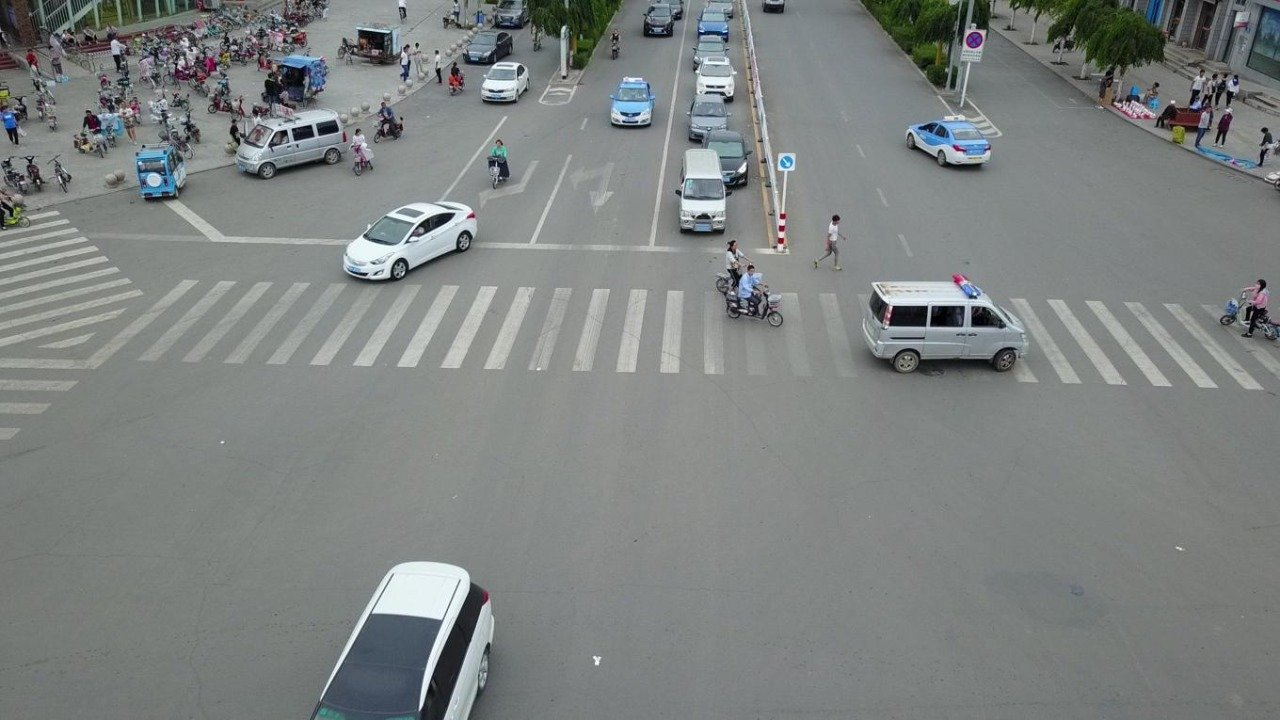
\includegraphics[width=\linewidth]{data_visdrone.jpg}\caption{VisDrone}\end{subfigure}\hfill
  \begin{subfigure}{0.32\linewidth}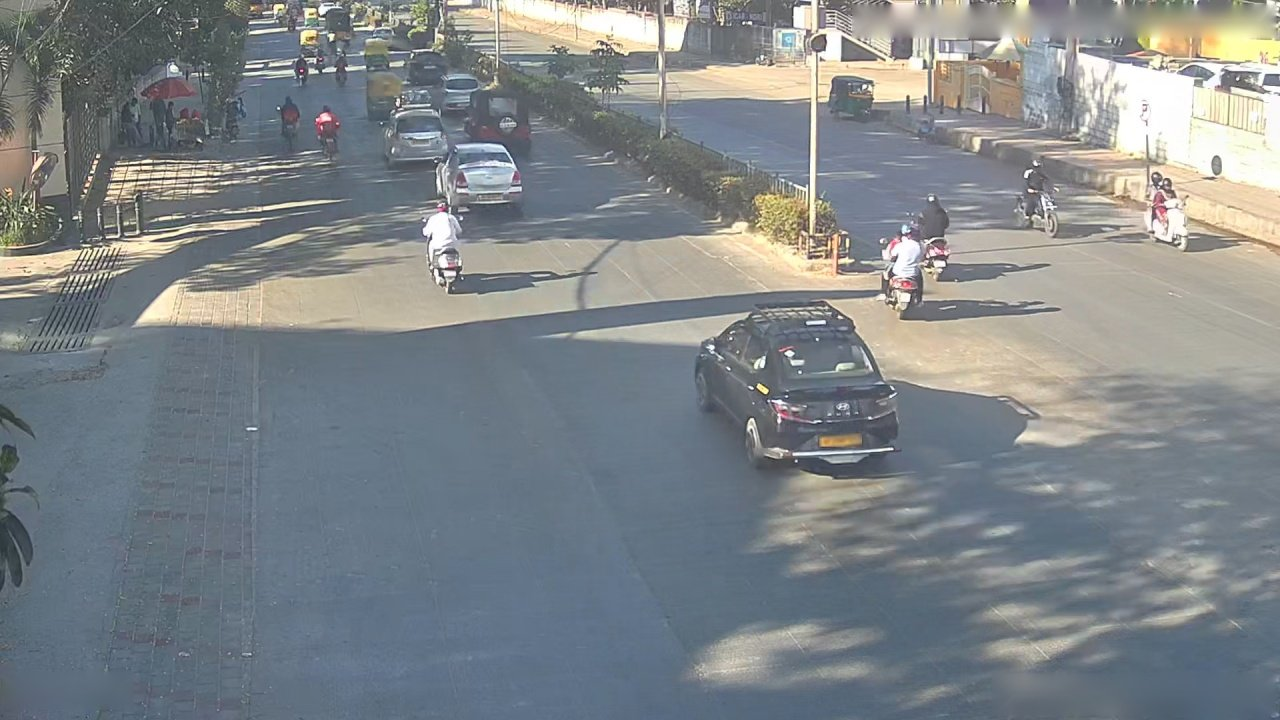
\includegraphics[width=\linewidth]{data_uvh26.jpg}\caption{UVH-26}\end{subfigure}\hfill
  \begin{subfigure}{0.32\linewidth}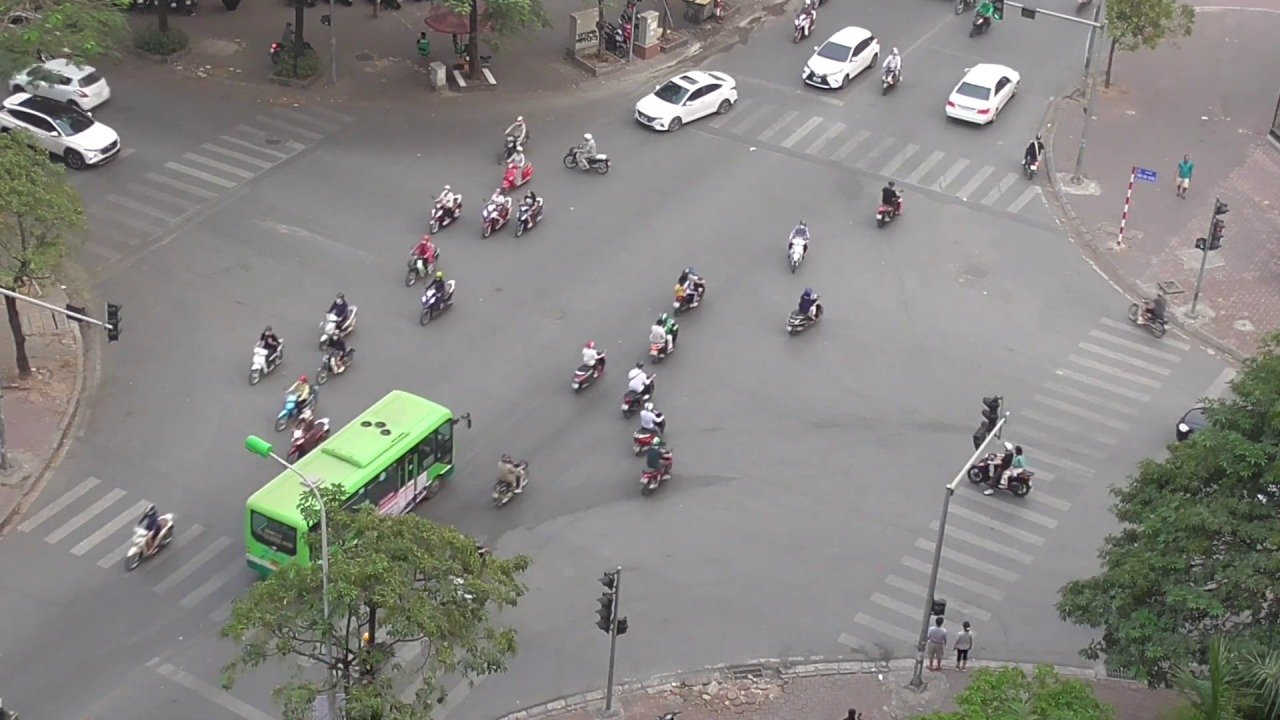
\includegraphics[width=\linewidth]{data_hanoi.jpg}\caption{Frame Hà Nội}\end{subfigure}
  \caption{Ví dụ ảnh từ sáu nguồn dữ liệu huấn luyện của v5}
  \label{fig:nguon-du-lieu}
\end{figure}

Lý do chọn từng nguồn gắn với các phiên bản mô hình ở mục~\ref{sec:cac-phien-ban}: VisDrone bù xe máy nhỏ nhìn từ trên
cao, frame Hà Nội bù đúng cảnh mục tiêu, UVH-26 là nguồn duy nhất đề tài tìm được có đúng góc camera giao thông trên
nhiều camera, còn frame đêm bù cảnh đường phố Việt Nam ban đêm (ví dụ ở Hình~\ref{fig:intro-traffic}b, phần Mở đầu).

\subsection{Chia tập huấn luyện, kiểm định và kiểm tra}
\label{sec:chia-tap}

Cách chia tập quyết định con số đánh giá có đáng tin hay không. Bộ \texttt{vehicle-vietnam-cantho} và
\texttt{vehicle-detection} gần như mỗi bộ chỉ có một camera, nếu chia ngẫu nhiên thì ảnh test và ảnh train là các frame
gần nhau của cùng một cảnh, mAP sẽ cao giả tạo. Vì vậy hai bộ này chỉ dùng để train. Tập val và test chỉ lấy từ bộ
\texttt{vietnamese-vehicle}, và đề tài không dùng cách chia sẵn của Roboflow. Các ảnh gần trùng nhau được gom thành nhóm
bằng mã băm cảm nhận dHash (hai ảnh có khoảng cách Hamming không quá 10 bit coi là cùng nhóm), rồi chia theo nhóm với
tỉ lệ 60/20/20 để không nhóm nào nằm ở hai tập. Ảnh được thu về cạnh dài tối đa 1280 điểm ảnh.

Frame Hà Nội được chia theo đoạn thời gian của video: 30 frame test lấy từ phút 0:35 đến 1:35 (mỗi 2 giây một frame),
10 frame val từ 1:45 đến 2:39, frame train lấy từ các đoạn sau đó. Cả ba phần đến từ \textbf{cùng một camera nhìn
xuống cùng một ngã tư}, chỉ khác thời điểm và mức zoom. Vì vậy với các mô hình đã học frame Hà Nội (v3 đến v6), tập test
Hà Nội đo độ chính xác \emph{trên chính camera đã dùng để tinh chỉnh}. Đây là một kịch bản triển khai có thật: camera
giao thông cố định, mô hình được tinh chỉnh bằng video của chính camera đó. Nhưng tập này không đo được khả năng tổng
quát sang camera mới. Khả năng tổng quát được đo trên các tập có camera không xuất hiện trong dữ liệu huấn luyện:
\texttt{vn\_extra}, clip Phạm Văn Đồng, val UVH-26 (đã bỏ ảnh cùng camera) và UA-DETRAC. Các clip Phạm Văn Đồng và hầm
chui chỉ dùng để test, không frame nào của chúng được đưa vào huấn luyện; frame đêm của v6 lấy từ hai camera khác.

Hai video đêm dùng để lấy frame huấn luyện là các đoạn ngắn được ghép lặp lại thành video dài (đoạn ở phút 15, phút 95
và phút 175 của một video có cùng nội dung). Frame được lấy 4 giây một lần trên mười đoạn hai phút, rồi bỏ những frame
gần trùng với frame đã lấy (chênh lệch điểm ảnh trung bình dưới 2 trên thang 0--255, sau khi thu nhỏ về 160×90; trên
video hầm chui, cặp frame trùng thật chênh 0.4--1.6). Các đoạn lặp lệch pha nhau nên bộ lọc chỉ bỏ 12 frame, còn 288
frame. Số cảnh giao thông thật sự khác nhau trong 288 frame này vì thế ít hơn con số 288.

Bảng~\ref{tab:thong-ke} là thống kê bộ dữ liệu phiên bản v6 (bản dùng cho mô hình triển khai): 5.002 ảnh train, 320 ảnh
val và 308 ảnh test. Bộ v5 giống hệt, chỉ thiếu dòng frame đêm (4.714 ảnh train).

\begin{table}[H]
  \centering
  \caption{Thống kê bộ dữ liệu v6 theo nguồn (số ảnh và số box mỗi lớp)}
  \label{tab:thong-ke}
  \small
  \begin{tabularx}{\linewidth}{|c|L|r|r|r|r|r|}
    \hline
    \thead{Tập} & \thead{Nguồn} & \thead{Ảnh} & \thead{Xe máy} & \thead{Ô tô} & \thead{Buýt} & \thead{Tải} \\ \hline
    train & cantho & 300 & 878 & 842 & 15 & 68 \\ \hline
    train & vehicle-detection & 300 & 2.181 & 844 & 49 & 51 \\ \hline
    train & vietnamese-vehicle & 929 & 1.328 & 1.629 & 197 & 1.123 \\ \hline
    train & VisDrone & 909 & 18.050 & 28.702 & 472 & 1.801 \\ \hline
    train & Hà Nội (69 frame × 4) & 276 & 18.192 & 4.256 & 68 & 100 \\ \hline
    train & UVH-26 & 2.000 & 12.348 & 7.066 & 1.231 & 3.351 \\ \hline
    train & Frame đêm (chỉ v6) & 288 & 6.256 & 3.811 & 162 & 148 \\ \hline
    val & vietnamese-vehicle & 310 & 451 & 579 & 93 & 352 \\ \hline
    val & Hà Nội & 10 & 889 & 156 & 7 & 1 \\ \hline
    test & vietnamese-vehicle & 308 & 453 & 609 & 115 & 303 \\ \hline
  \end{tabularx}
\end{table}

Xe máy và ô tô chiếm phần lớn số box; xe buýt và xe tải ít hơn nhiều. Đề tài không dùng trọng số lớp: mặc định của
Ultralytics không bật trọng số lớp, và trên tập test Roboflow (có nhiều buýt, tải) AP của hai lớp này không thấp hơn
xe máy (mục~\ref{sec:ket-qua-phat-hien}).

\subsection{Các tập đánh giá}
\label{sec:tap-danh-gia}

Tập test Roboflow không đại diện cho video mục tiêu (mục~\ref{sec:kho-khan}), nên đề tài tự xây thêm các tập đánh giá
Việt Nam và dùng thêm ba bộ dữ liệu bên ngoài (Bảng~\ref{tab:tap-danh-gia}).

\begin{table}[H]
  \centering
  \caption{Các tập đánh giá và vai trò (số box theo thứ tự xe máy / ô tô / buýt / tải)}
  \label{tab:tap-danh-gia}
  \small
  \begin{tabularx}{\linewidth}{|p{2.6cm}|L|p{2.9cm}|p{2.2cm}|}
    \hline
    \thead{Tập} & \thead{Nội dung} & \thead{Quy mô} & \thead{Vai trò} \\ \hline
    Val Hà Nội & 10 frame video ngã tư Hà Nội, nhãn người & 889 / 156 / 7 / 1 & Dev: chọn mô hình \\ \hline
    Test Hà Nội & 30 frame ngã tư Hà Nội, nhãn người (sơ bộ từ v2); cùng camera với frame train của v3--v6 & 2.982 /
      539 / 5 / 2 & Test phát hiện trên camera đã học \\ \hline
    \texttt{vn\_extra} ngày & 30 frame hai góc máy đại lộ Phạm Văn Đồng, nhãn người (sơ bộ từ YOLO26x) & 552 / 156 /
      0 / 2 & Test phát hiện \\ \hline
    \texttt{vn\_extra} đêm & 30 frame hầm chui TP.HCM ban đêm, nhãn người (sơ bộ từ YOLO26x) & 468 / 157 / 6 / 9 & Test
      phát hiện \\ \hline
    Dev đêm & 32 frame nút giao Công viên Gia Định (TP.HCM) ban đêm, YouTube kênh Vietnam Naturally; nhãn người (sơ bộ
      từ YOLO26x), 20 vùng bỏ qua; camera không có trong dữ liệu huấn luyện & 359 / 162 / 3 / 0 & Dev: nhận v6, chọn
      ngưỡng nhãn tự động ban đêm \\ \hline
    20 frame PVD & 1 frame mỗi giây của clip theo dõi & 375 / 238 / 12 / 0 & Test phát hiện \\ \hline
    Clip theo dõi PVD & 20 giây (600 frame, 30 fps), nhãn quỹ đạo bằng CVAT & 183 quỹ đạo & Test theo dõi, đếm xe
      ban ngày \\ \hline
    Đếm xe hầm chui & Hai clip đêm 60 giây, người đếm tay từng lượt qua vạch & 176 lượt: 149 / 25 / 1 / 1 & Test đếm xe
      ban đêm \\ \hline
    VnTraffic~\cite{le2026vntraffic} & Video giao thông Việt Nam (nguồn kênh HTV), nhìn chéo từ trên cao, 17 giây & 501
      frame, 85 quỹ đạo
      & Dev: chọn tracker \\ \hline
    Val UVH-26 & 509 ảnh, bỏ ảnh cùng camera với ảnh train & 2.973 / 1.239 / 219 / 546 & Chấm phụ \\ \hline
    UA-DETRAC~\cite{wen2020uadetrac, patrikskalos_uadetrac} & Camera cầu vượt Trung Quốc, 960×540; 21 video đêm và 39
      video ngày, 1 frame mỗi 100 frame & Đêm 51 / 1.578 / 143 / 21; ngày 35 / 4.003 / 246 / 19 & Chấm phụ đêm–ngày
      \\ \hline
    Test Roboflow & 308 ảnh \texttt{vietnamese-vehicle} & 453 / 609 / 115 / 303 & Chấm phụ \\ \hline
  \end{tabularx}
\end{table}

Ba tập dev được dùng để ra quyết định; mọi tập còn lại chỉ dùng để báo cáo. Một số lưu ý khi đọc các tập này:
\begin{itemize}
  \item \textbf{Val UVH-26.} UVH-26 chia train/val theo ảnh chứ không theo camera, nên đề tài lấy 800 ảnh val ngẫu
        nhiên rồi bỏ 291 ảnh có camera trùng với ảnh train đã dùng (so bằng dHash 256 bit, ngưỡng chọn bằng mắt), còn
        509 ảnh. Tập này đo khả năng tổng quát sang camera mới trong cùng miền Ấn Độ, không phải sang Việt Nam.
  \item \textbf{VnTraffic} là bộ nhãn theo dõi duy nhất tìm được đúng phạm vi, nhưng nhãn không đầy đủ: mỗi frame thiếu
        khoảng 6--9 xe mà mô hình phát hiện chắc chắn, và 55/85 quỹ đạo bị mất box 1--19 frame giữa chừng dù xe vẫn
        thấy rõ (đề tài lấp các khoảng này bằng box trung tính). Hệ quả là phát hiện thừa bị thổi phồng; trên tập này chỉ
        dùng AssA, IDR và số lần đổi ID để so tracker, vì ba chỉ số này không bị phạt khi phát hiện thêm xe.
  \item \textbf{UA-DETRAC} dùng bản nhãn gán lại có xe máy; điều kiện đêm hay ngày lấy theo thuộc tính thời tiết trong
        nhãn gốc (bỏ 11 video mưa). Đây là đường phố có đèn ở Trung Quốc, chủ yếu ô tô.
  \item \textbf{Dev đêm} được xây khi làm v6, vì hai tập dev cũ đều là cảnh ban ngày. Frame lấy 15 giây một lần từ bốn
        đoạn hai phút ở phút 40, 50, 58 và 64 của một video liền mạch, đều sau khi trời tối hẳn. Người gán thêm 248 box so với nhãn sơ bộ, phần lớn là
        xe máy nhỏ ở xa; 200 trong 524 xe cao dưới 32 điểm ảnh.
  \item \textbf{Video hầm chui.} Ba clip đêm được cắt ở ba thời điểm khác nhau của một video dài khoảng ba giờ, nhưng
        khi đếm xe từng frame mới thấy video gốc có đoạn lặp: frame 0--1387 của clip thứ nhất trùng frame 412--1799 của
        clip thứ hai (so chênh lệch điểm ảnh giữa các cặp frame), và clip thứ nhất có một chỗ cắt cảnh ở giây 48.3. Clip
        thứ hai và thứ ba liền mạch, không trùng nhau. Vì vậy tập \texttt{vn\_extra} đêm và phép đánh giá đếm xe ban đêm
        chỉ dùng clip thứ hai và thứ ba; clip thứ nhất chỉ để minh hoạ.
\end{itemize}

\section{Gán nhãn dữ liệu}

\subsection{Công cụ và quy trình}

Nhãn ảnh được gán bằng X-AnyLabeling, nhãn quỹ đạo video bằng CVAT. Gán từ đầu một frame có hơn 100 xe máy mất rất
nhiều thời gian, nên mọi tập đều theo quy trình ba bước: mô hình tạo nhãn sơ bộ, người gán sửa từng box, rồi một mô hình
khác rà soát để chỉ ra chỗ ``có thể sót'' và ``có thể thừa'' cho người gán xem lại.

Nhãn sơ bộ để lại dấu: box được người giữ nguyên mang cách khoanh của mô hình tạo ra nó. Với tập test Hà Nội, 69\% số
box là box sơ bộ của v2 giữ nguyên (IoU $\ge$ 0.95). Vì vậy với các tập test mới (\texttt{vn\_extra}), nhãn sơ bộ và rà
soát đều dùng YOLO26x gốc COCO, một mô hình không tham gia so sánh, để không ưu ái mô hình nào. Ảnh hưởng của dấu vết
này lên kết quả được bàn ở mục~\ref{sec:thao-luan}.

\subsection{Quy tắc gán nhãn}

\begin{itemize}
  \item Box xe máy bao cả người lái; xe bị che một phần được khoanh phần nhìn thấy.
  \item Chỉ gán nhãn một xe khi nhìn riêng frame đó xác định được đó là loại xe gì và nằm từ đâu đến đâu. Trường hợp mơ
        hồ (bị cây che gần hết, cụm xe quá xa) gán lớp \texttt{ignore} chứ không xoá, theo quy ước vùng bỏ qua của KITTI,
        COCO và VisDrone. Khi huấn luyện, box \texttt{ignore} bị bỏ vì Ultralytics không hỗ trợ vùng bỏ qua; khi chấm, chúng
        trở thành vùng \texttt{iscrowd}.
  \item \textbf{Xe van} được phân theo hình dáng thân xe, vì từ camera không biết xe chở người hay hàng: van nhỏ (Suzuki
        Blind Van, Towner, Tera V) và xe MPV 7 chỗ là ô tô; van cỡ Ford Transit mui cao, cả bản 16 chỗ lẫn bản chở hàng, là
        xe buýt. Quy tắc này khớp cách dữ liệu train v5 ánh xạ lớp (UVH-26 \texttt{Van} thành ô tô,
        \texttt{Tempo-traveller} và \texttt{Mini-bus} thành buýt). Nó lệch luật Việt Nam (van chở hàng là xe tải) và lệch
        KITTI, UA-DETRAC (có lớp van riêng), vì đề tài chỉ có bốn lớp.
  \item \textbf{Xe bán tải} năm chỗ (kiểu Ford Ranger) là ô tô. COCO xếp xe bán tải vào lớp xe tải, nhưng mọi mô hình
        của đề tài đều gọi loại xe này là ô tô, tức dữ liệu huấn luyện đã ngầm xếp nó vào ô tô, và ở Việt Nam xe bán tải
        chủ yếu dùng chở người. Theo quy ước COCO, hai lượt xe bán tải trong dữ liệu đếm ban đêm sẽ thành lỗi sai lớp
        của cả hai mô hình.
\end{itemize}

\subsection{Nhãn tự động cho frame huấn luyện}

69 frame train Hà Nội được gán nhãn tự động bằng cách ghép dự đoán của nhiều mô hình ``thầy'': v2 ở ảnh 960 và 1280,
YOLO26x ở ảnh 1280, và v2 chạy theo lát cắt SAHI~\cite{akyon2022sahi} 2×2 để bắt xe nhỏ; mỗi mô hình chạy thêm trên
ảnh lật ngang. Các box được ghép bằng Weighted Boxes Fusion~\cite{solovyev2021wbf}: box của các mô hình chồng lên nhau
được gộp thành một box có toạ độ là trung bình có trọng số theo điểm tin cậy. Box có điểm sau ghép từ 0.15 trở lên
được giữ; ngưỡng này chọn trên tập val Hà Nội có nhãn người, không nhìn tập test.

Đo trên val Hà Nội, nhãn tự động đạt Precision 0.905, Recall 0.853, F1 0.878; recall của xe máy là 0.841, cao hơn bản
không dùng SAHI (0.802). Phần bị sót chủ yếu là cụm xe máy dừng đèn đỏ.

288 frame đêm của v6 được gán nhãn theo cùng cách, với bộ thầy mạnh hơn: RT-DETRv2-S ở ảnh 960 (quá chậm để triển khai
nhưng dùng làm thầy được), YOLO26x ở ảnh 1280, v5 ở ảnh 960 và 1280, và v5
chạy theo lát cắt 2×2. Ngưỡng giữ box được chọn trên tập dev đêm (32 frame nhãn người, camera không có trong
frame train). Trên tập này, bản thêm lát cắt 2×2 cho mAP50 chính 0.800, cao hơn bản không cắt (0.778) và cao hơn thầy
mạnh nhất đứng riêng (RT-DETRv2-S, 0.702). F1 cao nhất là 0.712 ở ngưỡng 0.20 (Precision 0.81, Recall 0.63), nên ngưỡng
0.20 được dùng. Nhãn đêm thiếu nhiều hơn nhãn Hà Nội: xe cao từ 64 điểm ảnh trở lên được giữ khoảng 95\%, nhưng xe cao
dưới 32 điểm ảnh chỉ khoảng 40\%. Phần xe nhỏ bị sót trong nhãn là rủi ro của v6, vì mô hình có thể học rằng xe nhỏ ở
xa là nền; tiêu chí nhận v6 (mục~\ref{sec:tieu-chi-chon}) được đặt để phát hiện trường hợp đó.

\subsection{Bổ sung nhãn UVH-26}

Khi kiểm tra UVH-26, đề tài thấy nhãn thiếu ít nhất 15\% số xe, chủ yếu xe ở xa. Nhãn thiếu làm mô hình học rằng xe ở xa
là nền. Đề tài bổ sung bằng YOLO26x: dự đoán có điểm từ 0.5 trở lên ở chỗ chưa có box được thêm vào; dự đoán nằm quá
50\% trong một box đã có (kể cả box của lớp bị bỏ như xe ba bánh) bị loại để không tạo box trùng.

\subsection{Nhãn quỹ đạo cho clip test}

Clip test theo dõi dài 20 giây (giây 20--40 của clip \texttt{pvd\_goc\_a}, 600 frame). Nhãn sơ bộ là quỹ đạo do chính
tracker sinh ra, xuất sang CVAT với keyframe mỗi 10 frame; người gán kiểm từng quỹ đạo, sửa box và ID. Sau đó nhãn
được soát lại mà không dùng mô hình của đề tài: dải xa phía trên ảnh (toạ độ y nhỏ hơn 462, nơi xe máy cao dưới 25 điểm
ảnh theo ngưỡng của KITTI) là vùng bỏ qua; 20 quỹ đạo được kéo dài tới dải đó bằng so khớp mẫu; 14 chỗ quỹ đạo bị đứt
oan được nối lại; 121 box ``mảnh vụn'' của xe khuất sau cây được chuyển sang trạng thái không hiện diện sau khi xem
bằng mắt.
YOLO26x chỉ dùng để soát chéo. Mọi chỉnh sửa và lý do được ghi lại để truy ngược. Kết quả là 183 quỹ đạo.

\subsection{Nhãn đếm xe ban đêm}
\label{sec:nhan-dem}

Hai clip hầm chui chưa có nhãn quỹ đạo, nên số lượt xe thật được đếm tay trên video gốc, không hiện kết quả của mô hình.
Đây cũng là cách cuộc thi AI City Challenge tạo nhãn cho bài đếm xe. Đề tài viết một công cụ nhỏ: video phát chậm
0.25 lần, có vẽ vạch đếm (nằm ngang ở 60\% chiều cao ảnh, trùng vạch của hệ thống); mỗi khi điểm giữa đáy xe chạm vạch,
người đếm bấm một phím theo lớp và hướng, công cụ ghi lại frame đang hiện. Xe đã ở phía trên vạch khi clip bắt đầu, hoặc
chưa tới vạch khi clip kết thúc, không được tính. Bộ đếm của hệ thống cũng lấy điểm giữa đáy box làm điểm neo, nên
người đếm và hệ thống đo cùng một sự kiện.

Để kiểm tra độ tin cậy của nhãn, một trợ lý AI đếm độc lập trên cùng hai clip bằng cách xem ảnh gốc, không dùng mô hình
của đề tài. Hai bộ đếm ghép được 174 trên 176 lượt (lệch thời điểm trung vị 0.2 giây); trong đó chỉ hai lượt khác lớp,
đều là xe bán tải mà bộ đếm AI xếp vào xe tải theo COCO. Hai lượt còn lại là hai xe máy ở giây cuối của clip thứ ba mà
bộ đếm AI chưa chốt; xem phóng to các frame cuối cho thấy cả hai đều qua vạch trước khi clip kết thúc, nên được giữ theo
người đếm. Kết quả là 176 lượt, cùng một chiều: 149 xe máy, 25 ô tô, 1 xe buýt, 1 xe tải.

\section{Huấn luyện mô hình phát hiện}

\subsection{Cấu hình huấn luyện}

Mọi mô hình được huấn luyện trên GPU Tesla T4 của Kaggle, khởi tạo từ trọng số đã huấn luyện trên COCO. Cấu hình chung
cho YOLO26:
\begin{itemize}
  \item tối đa 100 epoch, dừng sớm nếu mAP50-95 trên val không tăng sau 20 epoch; seed 42 (để đo dao động giữa các lần
        huấn luyện, v5 và YOLO26s được huấn luyện thêm với seed 1 và 2, v6 với seed 1);
  \item kích thước ảnh 960 (v1 dùng 640, v4 dùng 1280); batch 16, cộng dồn gradient tới batch danh nghĩa 64;
  \item optimizer chọn tự động: số vòng lặp dự kiến với bộ dữ liệu v5 là $\lceil 4714 / 64 \rceil \times 100 = 7.400$,
        với v6 là $\lceil 5002 / 64 \rceil \times 100 = 7.900$, đều dưới 10.000, nên Ultralytics chọn AdamW với tốc độ
        học 0.00125;
  \item tăng cường dữ liệu mặc định (ghép 4 ảnh mosaic, đổi màu HSV, lật, co giãn, dịch), tắt mosaic ở 10 epoch cuối;
  \item lưu trọng số trung bình trượt EMA; chọn checkpoint có mAP50-95 val cao nhất; huấn luyện độ chính xác hỗn hợp.
\end{itemize}

\subsection{Quá trình cải tiến qua các phiên bản}
\label{sec:cac-phien-ban}

Mô hình được cải tiến qua sáu phiên bản dữ liệu, mỗi lần chỉ đổi một yếu tố để biết thay đổi nào có tác dụng
(Bảng~\ref{tab:lich-su-train}).

\begin{table}[H]
  \centering
  \caption{Lịch sử huấn luyện các mô hình (val và test Roboflow do bộ chấm của thư viện tính khi train)}
  \label{tab:lich-su-train}
  \footnotesize
  \begin{tabularx}{\linewidth}{|p{1.5cm}|L|>{\centering\arraybackslash}p{0.8cm}|>{\centering\arraybackslash}p{1.5cm}|>{\centering\arraybackslash}p{1.7cm}|>{\centering\arraybackslash}p{1.8cm}|>{\centering\arraybackslash}p{0.9cm}|}
    \hline
    \thead{Mô hình} & \thead{Dữ liệu train} & \thead{Ảnh} & \thead{Epoch tốt nhất / đã chạy} &
      \thead{Val mAP50 / 50-95} & \thead{Test Roboflow mAP50 / 50-95} & \thead{Giờ T4} \\ \hline
    v1 & Roboflow + VisDrone & 640 & 81 / 100 & 0.831 / 0.549 & 0.861 / 0.572 & 0.84 \\ \hline
    v2 & cantho, vehicle-detection 300 ảnh mỗi bộ; VisDrone 909 ảnh nhiều xe máy & 960 & 86 / 100 & 0.838 / 0.555 &
      0.864 / 0.573 & 1.61 \\ \hline
    v3 & v2 + 69 frame Hà Nội nhãn tự động + 10 frame val & 960 & 80 / 100 & 0.853 / 0.616 & 0.870 / 0.573 & 1.79 \\ \hline
    v4 & như v3 & 1280 & 83 / 100 & 0.851 / 0.616 & 0.873 / 0.575 & 3.18 \\ \hline
    v5 & v3 + 2.000 ảnh UVH-26 & 960 & 90 / 100 & 0.867 / 0.628 & 0.861 / 0.578 & 2.96 \\ \hline
    v5, seed 1 & như v5 & 960 & 69 / 89 & 0.877 / 0.638 & 0.868 / 0.590 & 2.68 \\ \hline
    v5, seed 2 & như v5 & 960 & 93 / 100 & 0.871 / 0.630 & 0.862 / 0.579 & 3.02 \\ \hline
    \textbf{v6} & v5 + 288 frame đêm nhãn tự động & 960 & 73 / 93 & 0.868 / 0.629 & 0.868 / 0.584 & 3.04 \\ \hline
    v6, seed 1 & như v6 & 960 & 85 / 100 & 0.862 / 0.626 & 0.858 / 0.587 & 3.27 \\ \hline
    YOLO26s & như v5 & 960 & 87 / 100 & 0.873 / 0.639 & 0.884 / 0.600 & 4.90 \\ \hline
    YOLO26s, seed 1 & như v5 & 960 & 81 / 100 & 0.875 / 0.644 & 0.879 / 0.594 & 5.36 \\ \hline
    YOLO26s, seed 2 & như v5 & 960 & 60 / 80 & 0.873 / 0.647 & 0.887 / 0.603 & 4.31 \\ \hline
    RT-DETRv2-S & như v5 & 960 & 61 / 81 & 0.878 / 0.651 & 0.874 / 0.601 & 10.7 \\ \hline
  \end{tabularx}
\end{table}

Lý do của từng bước:
\begin{itemize}
  \item \textbf{v1} đạt mAP50 0.861 trên test Roboflow, nhưng trên frame Hà Nội gần như không bắt được xe máy (AP50 xe
        máy 0.045), còn kém mô hình gốc COCO. Tập test Roboflow không đại diện cho cảnh mục tiêu, nên từ đây mọi mô
        hình đều được chấm thêm trên frame Việt Nam tự gán.
  \item \textbf{v2} tăng kích thước ảnh lên 960 và thêm ảnh VisDrone có nhiều xe máy nhỏ nhìn từ trên cao. Trên 5
        frame Hà Nội, v2 bắt được 405 xe máy so với 167 của mô hình COCO ở ảnh 1280 và 12 của v1.
  \item \textbf{v3} thêm frame Hà Nội gán nhãn tự động, tức đúng cảnh mục tiêu (lặp 4 lần để đủ trọng số).
  \item \textbf{v4} thử tăng ảnh lên 1280. Trên val Hà Nội không tốt hơn v3 (0.916 so với 0.917) mà chậm hơn, nên giữ v3.
  \item \textbf{v5} thêm 2.000 ảnh UVH-26 có đúng góc camera giao thông. Khi phân tích các xe v3 bỏ sót trên VnTraffic
        (một xe buýt bị che một phần, một xe tải nhìn xiên, xe máy dừng nhìn thẳng), đề tài thấy v3 không nhận ra chúng ở
        mọi kích thước ảnh, trong khi dữ liệu train đã có hàng trăm xe buýt và hàng nghìn xe tải. Nguyên nhân là thiếu ảnh
        đúng góc camera giao thông chứ không thiếu lớp; v5 nhận ra được các xe này.
  \item \textbf{v6} thêm 288 frame đêm từ hai camera mới, gán nhãn tự động. Hướng này xuất phát từ kết quả của v5: ban
        đêm là cảnh v5 yếu nhất và dao động mạnh nhất giữa các lần huấn luyện (mục~\ref{sec:thao-luan}). Frame đêm lấy từ camera
        khác với clip hầm chui dùng để test.
\end{itemize}

Hai mô hình YOLO26s và RT-DETRv2-S dùng đúng dữ liệu v5 để so sánh kiến trúc (mục~\ref{sec:giao-thuc}). Hình~\ref{fig:hoc}
là đường học trên tập val của ba mô hình cùng dữ liệu v5. RT-DETRv2-S hội tụ sớm hơn, gần như không tăng từ khoảng
epoch 55, nên bị dừng sớm ở epoch 81, trước pha tắt tăng cường dữ liệu ở 10 epoch cuối mà hai bản YOLO đều trải qua.

\begin{figure}[H]
  \centering
  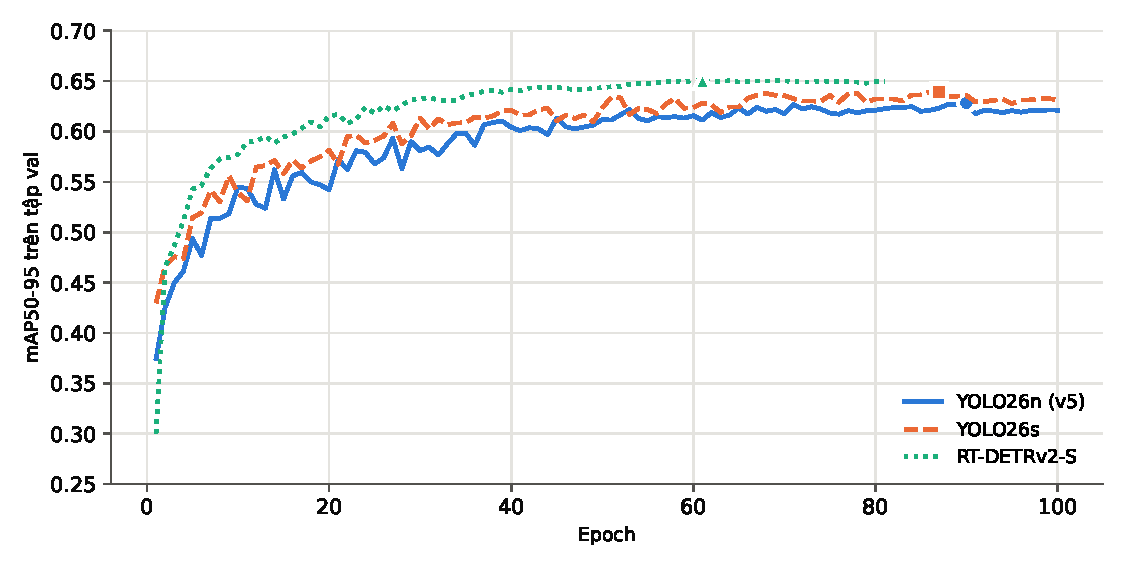
\includegraphics[width=0.92\linewidth]{learning_curves.pdf}
  \caption{mAP50-95 trên tập val theo epoch của ba mô hình huấn luyện trên dữ liệu v5; điểm đánh dấu là epoch được
           chọn. Số của YOLO do bộ chấm Ultralytics tính, số của RT-DETRv2 do pycocotools tính, nên chỉ so được hình
           dạng đường học}
  \label{fig:hoc}
\end{figure}

\subsection{Tiêu chí chọn mô hình}
\label{sec:tieu-chi-chon}

Tiêu chí được đặt trước khi chạy: với mô hình phát hiện, so mAP50 chính trên val Hà Nội; với tác động lên theo dõi, so
IDR trên VnTraffic; chênh lệch dưới 0.005 điểm là hoà và khi hoà chọn phương án nhanh hơn. Theo tiêu chí này:
\begin{itemize}
  \item \textbf{v5 được chọn thay v3}: mAP50 val hoà (0.919 so với 0.917) nhưng trên VnTraffic IDR tăng từ 0.744 lên
        0.827 và số lần đổi ID giảm từ 128 xuống 62. Hai lần huấn luyện lại v5 với seed khác sau đó cho cùng kết luận
        (mục~\ref{sec:thao-luan}).
  \item \textbf{Giữ ảnh 960 cho v5}, không dùng 1280: mAP50 val hoà (0.922 so với 0.919), trên VnTraffic bản 1280 đổi
        ID nhiều hơn (85 so với 62) và chậm hơn khoảng 1.5 lần.
\end{itemize}

Với v6, vì độ chính xác ban đêm dao động mạnh giữa các lần huấn luyện, tiêu chí được viết ra trước khi huấn luyện v6
và tính trên cả hai lần huấn luyện (seed 42 và 1), so với ba lần huấn luyện của v5. v6 được nhận nếu đạt đủ ba điều
kiện; nếu không, giữ v5 và báo cáo kết quả âm tính. Kết quả:
\begin{enumerate}
  \item mAP50 chính trên dev đêm của cả hai lần v6 phải cao hơn lần tốt nhất của v5 (0.499; ba lần v5 đạt 0.499, 0.498
        và 0.464): v6 đạt 0.599 và 0.618, \textbf{đạt}.
  \item mAP50 chính trên val Hà Nội của mỗi lần v6 không thấp hơn lần kém nhất của v5 quá 0.005 (tức từ 0.909 trở lên):
        cả hai lần đạt 0.914, \textbf{đạt}.
  \item IDR trên VnTraffic của mỗi lần v6 không thấp hơn lần kém nhất của v5 quá 0.005 (từ 0.822 trở lên): 0.841 và
        0.824, \textbf{đạt}, lần thứ hai sát ngưỡng.
\end{enumerate}
Mô hình triển khai là \textbf{v6 với seed 42}, theo cùng quy ước với các phiên bản trước; lần huấn luyện với seed 1 chỉ
dùng để đo độ dao động.

\section{Giao thức so sánh kiến trúc CNN và Transformer}
\label{sec:giao-thuc}

Câu hỏi của thí nghiệm là: họ Transformer có phát hiện xe Việt Nam tốt hơn họ CNN không, và phải trả bao nhiêu về tốc
độ. Nguyên tắc là đồng nhất mọi yếu tố đồng nhất được mà không làm bên nào bị huấn luyện sai công thức của nó; yếu tố
nào gắn với kiến trúc thì mỗi bên giữ theo bản chính thức và ghi rõ. YOLO26 dùng mặc định của Ultralytics 8.4.163;
RT-DETRv2-S dùng cấu hình chính thức của tác giả cho bản ResNet-18, chạy qua thư viện Transformers.

\begin{table}[H]
  \centering
  \caption{Các yếu tố được đồng nhất giữa YOLO26 và RT-DETRv2-S}
  \label{tab:dong-nhat}
  \small
  \begin{tabularx}{\linewidth}{|p{4cm}|L|}
    \hline
    \thead{Yếu tố} & \thead{Cách giữ đồng nhất} \\ \hline
    Dữ liệu và nhãn & Cùng bộ v5 (4.714 train, 320 val, 308 test), cùng file nhãn \\ \hline
    Khởi tạo & Cả hai từ trọng số COCO, đầu phân lớp khởi tạo lại cho 4 lớp \\ \hline
    Kích thước ảnh & 960 \\ \hline
    Số epoch, dừng sớm & Tối đa 100; dừng khi mAP50-95 val không tăng sau 20 epoch \\ \hline
    Chọn checkpoint & Trọng số EMA có mAP50-95 val cao nhất; cùng công thức EMA \\ \hline
    Optimizer & AdamW ở cả hai; huấn luyện độ chính xác hỗn hợp; seed 42 \\ \hline
    Đầu ra & Tối đa 300 phát hiện mỗi ảnh, không NMS, không TTA \\ \hline
    Chấm điểm & Một đường chấm chung: pycocotools, ngưỡng tin cậy 0.001, tối đa 500 phát hiện mỗi ảnh, cùng vùng bỏ
      qua, cùng bootstrap \\ \hline
    Đo tốc độ và độ phức tạp & Cùng CPU, cùng frame, cùng giao diện (tiền xử lý + suy luận + hậu xử lý); GFLOPs đo bằng
      cùng công cụ ở đúng đầu vào thực tế \\ \hline
  \end{tabularx}
\end{table}

Ba yếu tố của RT-DETRv2 được chỉnh lệch bản chính thức cho giống YOLO: kích thước ảnh 640 thành 960; warmup tốc độ học
2.000 bước thành 3 epoch (2.000 bước là khoảng 0.27 epoch trên COCO nhưng gần 7 epoch trên 4.714 ảnh); tắt tăng cường
dữ liệu mạnh ở 10 epoch cuối thay vì 3.

Các yếu tố không thể đồng nhất vì gắn với công thức của từng họ được liệt kê trong Bảng~\ref{tab:khong-dong-nhat}.

\begin{table}[H]
  \centering
  \caption{Các yếu tố khác nhau giữa hai họ mô hình}
  \label{tab:khong-dong-nhat}
  \small
  \begin{tabularx}{\linewidth}{|p{2.8cm}|L|L|}
    \hline
    \thead{Yếu tố} & \thead{YOLO26} & \thead{RT-DETRv2-S} \\ \hline
    Tốc độ học & 0.00125, giảm tuyến tính & $10^{-4}$ cố định sau warmup, cắt gradient 0.1 \\ \hline
    Batch hiệu dụng & 64 (batch 16 hoặc 8, cộng dồn gradient) & 16 (8 × cộng dồn 2) \\ \hline
    Tăng cường dữ liệu & Mosaic, HSV, lật, co giãn & Biến đổi màu, ZoomOut, IoUCrop, lật \\ \hline
    Đưa ảnh về 960 & Giữ tỉ lệ, đệm viền: video 1080p thành 544×960 & Kéo giãn thành 960×960 \\ \hline
    Mất mát & BCE, box IoU, L1 & VFL, L1, GIoU, denoising \\ \hline
  \end{tabularx}
\end{table}

Batch không được ép bằng nhau vì nó gắn chặt với tốc độ học của từng công thức. Nếu ép YOLO về batch danh nghĩa 16, số
vòng lặp vượt 10.000 và Ultralytics tự đổi sang optimizer MuSGD với tốc độ học 0.01, tức YOLO bị huấn luyện theo công
thức khác. Hệ quả cần nhớ khi đọc kết quả: với video 16:9, YOLO nhìn 960×540 điểm ảnh có nội dung còn RT-DETRv2 nhìn
960×960, nhiều hơn khoảng 1.8 lần. Vì vậy đề tài chạy thêm một đối chứng: YOLO26s ở ảnh 1280 (1280×720 bằng khoảng
960×960 điểm ảnh).

Trước khi chấm chính thức, đường chấm được kiểm chứng trên 320 ảnh val. Với RT-DETRv2, đường chấm của đề tài cho mAP50
0.8785 và mAP50-95 0.6506, lệch dưới 0.001 so với nhật ký huấn luyện. Với YOLO26s, số thư viện in khi train (0.873)
cao hơn đường chấm của đề tài (0.847); nguyên nhân là chế độ chấm của Ultralytics đệm thêm viền ảnh. Khi chấm chính dự
đoán của Ultralytics bằng bộ chấm của đề tài thì ra 0.870, khớp 0.872, nên bộ chấm đúng. Đường chấm của đề tài đo đúng
cách mô hình chạy khi triển khai và áp dụng như nhau cho mọi mô hình.

\section{Theo dõi đối tượng và chọn tracker}
\label{sec:chon-tracker}

Đánh giá theo dõi dùng hai tập tách biệt: VnTraffic là tập dev để chọn tracker và chỉnh tham số; clip Phạm Văn Đồng
gán nhãn tay là tập test, dùng để chấm cấu hình đã chọn. Việc chấm không phân lớp (mọi xe là một lớp), vì tracker của
Ultralytics ghép box chỉ theo vị trí, không xét lớp; chất lượng phân loại đã được đo bằng mAP.

Quá trình chọn gồm bốn bước, kết quả chi tiết ở mục~\ref{sec:theo-doi}:
\begin{enumerate}
  \item So ByteTrack, BoT-SORT và OC-SORT với tham số mặc định: BoT-SORT tốt nhất trên cả AssA, IDR và số lần đổi ID.
  \item Chỉnh lưới tham số BoT-SORT (thời gian giữ track mất 30, 60 hay 90 frame; bật hay tắt ReID): chọn giữ track 90
        frame, không ReID. Bật ReID bằng đặc trưng của chính mô hình phát hiện làm số lần đổi ID tăng từ 128 lên khoảng
        208.
  \item Tắt bù chuyển động camera (GMC): camera trong phạm vi đề tài đứng yên, GMC chỉ ước lượng chuyển động gần bằng 0
        mà tốn thời gian; trên dev hai bản hoà nhau nên chọn bản nhanh hơn.
  \item Trong pipeline video, bỏ các track tồn tại dưới 3 frame (tương đương \texttt{min\_hits} của SORT) để giảm track
        rác; bộ chấm vẫn báo kết quả thô làm số chính.
\end{enumerate}

\begin{table}[H]
  \centering
  \caption{Cấu hình tracker mặc định của hệ thống (BoT-SORT đã chỉnh, không GMC)}
  \label{tab:tracker-config}
  \small
  \begin{tabularx}{\linewidth}{|p{4.2cm}|c|L|}
    \hline
    \thead{Tham số} & \thead{Giá trị} & \thead{Ý nghĩa} \\ \hline
    \texttt{track\_high\_thresh} & 0.25 & Ngưỡng box điểm cao cho lần ghép thứ nhất \\ \hline
    \texttt{track\_low\_thresh} & 0.1 & Ngưỡng dưới của box dùng ở lần ghép thứ hai \\ \hline
    \texttt{new\_track\_thresh} & 0.25 & Điểm tối thiểu để tạo track mới \\ \hline
    \texttt{track\_buffer} & 90 & Số frame giữ track bị mất trước khi xoá \\ \hline
    \texttt{match\_thresh} & 0.8 & Ngưỡng chi phí ghép cặp \\ \hline
    \texttt{gmc\_method} & none & Tắt bù chuyển động camera \\ \hline
    \texttt{with\_reid} & false & Không dùng đặc trưng ngoại hình \\ \hline
  \end{tabularx}
\end{table}

\section{Pipeline hệ thống và ứng dụng}

\subsection{Luồng xử lý}

Hình~\ref{fig:pipeline} là luồng xử lý mỗi frame. Toàn bộ logic nằm trong một hàm dùng chung cho chương trình dòng lệnh,
web demo và bộ chấm theo dõi, nên số liệu đo được đúng là thứ chạy trong demo.

\begin{figure}[H]
  \centering
  % Vẽ bằng TikZ ở report/figures_src/pipeline.tex, biên dịch sẵn thành PDF cho nhanh
  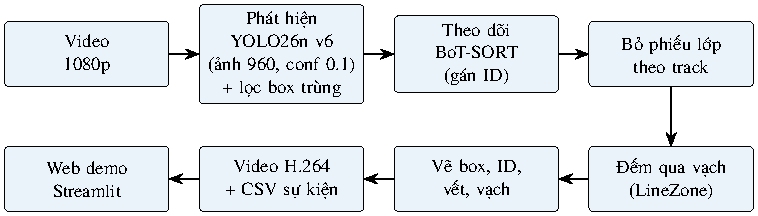
\includegraphics[width=\linewidth]{pipeline.pdf}
  \caption{Luồng xử lý của hệ thống}
  \label{fig:pipeline}
\end{figure}

Các bước:
\begin{enumerate}
  \item \textbf{Phát hiện và theo dõi.} Mỗi frame được đưa qua mô hình phát hiện với ngưỡng tin cậy 0.1 rồi qua BoT-SORT.
        Ngưỡng 0.1 để tracker có box điểm thấp cho lần ghép thứ hai; việc tạo track mới do \texttt{new\_track\_thresh}
        (0.25) quyết định. Ở frame đầu của mỗi video tracker được tạo mới, để chạy nhiều video liên tiếp trong web demo
        không bị dính ID cũ.
  \item \textbf{Ánh xạ lớp theo tên.} Tên lớp của mô hình được đổi sang bốn lớp chuẩn theo tên (ví dụ
        \texttt{motorcycle} thành \texttt{motorbike}), nên cùng một mã chạy được với mô hình COCO gốc và các mô hình
        tinh chỉnh.
  \item \textbf{Bỏ phiếu lớp theo track.} Một xe có thể bị gọi lúc là ô tô, lúc là xe tải giữa các frame. Lớp của mỗi
        track được chọn bằng bỏ phiếu có trọng số độ tin cậy:
\end{enumerate}
\begin{equation}
  \hat{c}(k) = \arg\max_{c} \sum_{t \in \mathcal{T}_k} s_t \cdot \mathbf{1}\{c_t = c\}
  \label{eq:vote}
\end{equation}
Công thức (\ref{eq:vote}): lớp của track $k$, với $\mathcal{T}_k$ là các frame track $k$ xuất hiện, $c_t$ và $s_t$ là
lớp và điểm tin cậy của box ở frame $t$. Lớp sau bỏ phiếu được ghi đè lên kết quả trước khi đếm, vì thư viện đếm theo lớp
tại thời điểm xe cắt vạch.
\begin{enumerate}[resume]
  \item \textbf{Đếm qua vạch.} Vạch đếm là một đoạn thẳng do người dùng đặt (mặc định nằm ngang ở 60\% chiều cao ảnh).
        Điểm giữa cạnh đáy của box được dùng làm điểm neo; khi điểm neo của một track đi từ bên này sang bên kia vạch,
        hệ thống ghi một sự kiện gồm frame, thời điểm, ID, lớp và hướng (vào hoặc ra).
  \item \textbf{Hiển thị và xuất kết quả.} Box được vẽ theo màu lớp, nhãn ``\#ID lớp'' chỉ ghi cho xe cao từ 4\% khung
        hình trở lên (xe nhỏ ở xa chỉ vẽ khung để chữ không đè nhau). ID hiển thị được đánh lại 1, 2, 3, \ldots theo thứ
        tự xe xuất hiện, vì ID gốc của tracker lên tới hàng nghìn do các track thử nghiệm bị huỷ vẫn tiêu số. Video được
        mã hoá lại sang H.264 để trình duyệt phát được; danh sách sự kiện xuất ra file CSV, kèm file cấu hình đã dùng.
\end{enumerate}

\subsection{Web demo và triển khai}

Web demo viết bằng Streamlit có hai chế độ. Chế độ chạy trực tiếp cho chọn clip có sẵn hoặc tải video lên, chọn mô hình,
tracker, ngưỡng tin cậy và vị trí vạch đếm, rồi hiển thị video kết quả, bảng đếm theo lớp và hướng, biểu đồ số xe cộng
dồn theo thời gian và cho tải file CSV. Chế độ thứ hai nạp lại video đã xử lý sẵn trên GPU, dùng khi trình chiếu vì
trên laptop, tính cả vẽ kết quả và ghi video 1080p, cả quy trình chỉ đạt khoảng 7 frame/s.

Để chạy nhanh trên laptop, mô hình triển khai được xuất sang OpenVINO~\cite{openvino}. Bản dùng cho web demo nhận ảnh
544×960, đúng khung video 16:9 với cạnh dài bằng kích thước ảnh lúc huấn luyện, và chạy trên GPU Intel tích hợp của
laptop. Cấu hình này được chọn khi v5 còn là mô hình triển khai; cách chọn và các phương án khác (INT8, chạy trên CPU)
trình bày ở mục~\ref{sec:openvino}. v6 dùng lại đúng cấu hình đó, vì cùng kiến trúc và cùng kích thước đầu vào.

\section{Kết luận chương}

Chương này đã trình bày cách xây dựng hệ thống. Dữ liệu huấn luyện gộp từ bảy nguồn, chia theo cảnh để tránh rò rỉ giữa
train và test; các tập đánh giá Việt Nam do đề tài tự gán nhãn, gồm cả cảnh đêm, một clip có nhãn quỹ đạo và hai clip
đêm có số lượt qua vạch do người đếm tay. Mô hình phát hiện được cải tiến qua sáu phiên bản dữ liệu, chọn bằng tiêu chí
đặt trước trên tập dev, và mô hình triển khai là YOLO26n v6, xuất sang OpenVINO để chạy trên GPU tích hợp của laptop.
Thí nghiệm so sánh với RT-DETRv2-S theo một giao thức ghi rõ các yếu tố đồng nhất và không đồng nhất được. Thuật toán
theo dõi được chọn là BoT-SORT đã chỉnh, không bù chuyển động camera. Chương~\ref{chap:ketqua} trình bày kết quả thực
nghiệm của các lựa chọn này.
